\documentclass{article}
\setlength\topmargin{0pt}
\addtolength\topmargin{-\headheight}
\addtolength\topmargin{-\headsep}
\setlength\oddsidemargin{0pt}
\setlength\textwidth{\paperwidth}
\addtolength\textwidth{-2in}
\setlength\textheight{\paperheight}
\addtolength\textheight{-2in}
\usepackage{layout}
\usepackage{amsmath}
\usepackage{algorithm}
\usepackage{verbatim}
\usepackage[noend]{algpseudocode}
\usepackage{graphicx}
\graphicspath{ {./} }


\title{\vspace{-2.0cm}CS M152A Project 2 Report}
\author{Melody Chen}

\begin{document}
\maketitle
\section{Introduction and Requirement} 
The focus of this lab is for students to learn how to use the Xilinx ISE software to design and test a floating point converter. To implement the floating point converter, we build a combinational circuit that that receives a 13-bit linear encoding of an analog signal and outputs a compounded 9-bit Floating Point(FP) Representation. For the output, we use a simplified Floating Point Representation consisting of 1-Bit Sign Representation($S$), a 3-Bit Exponent($E$), and a 5-Bit Significand($F$). The value represented by our simplified FP can be calculated by:
\begin{center}
    $V = (-1)^{S} * F * 2^{E}$
\end{center}
Part of the focus of this lab is to take care of rounding for cases we cannot accurately represent in our FP format and to ensure that we have correct FP representation for all edge cases. More details about rounding will be explained in later parts of the report. After implementing the floating point conversion module, we design a test bench and simulate the behaviors of varying inputs to show the accuracy of our module. 
\section{Design Description}
For the design and implementation of the floating point converter circuit, I followed the overall block diagram provided in the project description, shown below:
\begin{center}
    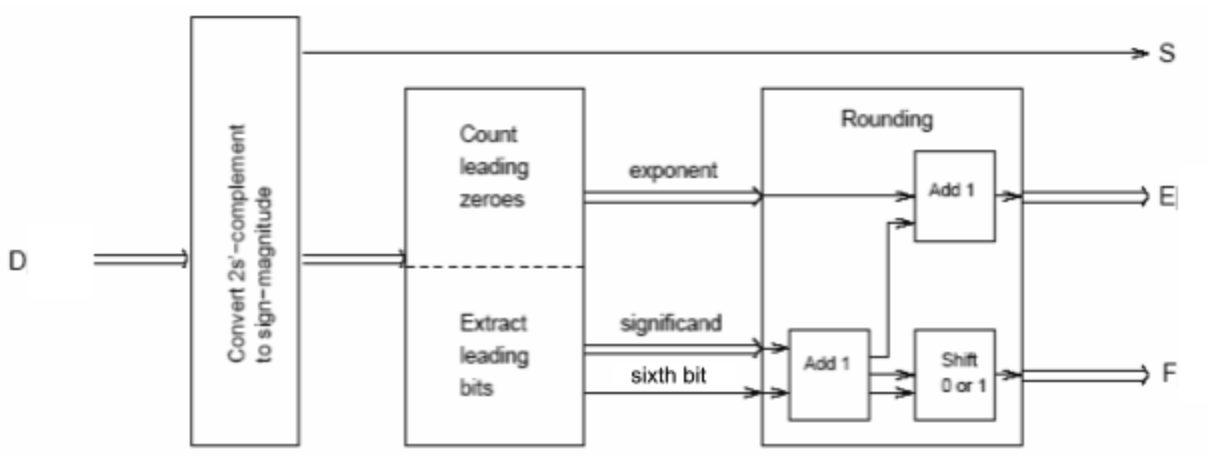
\includegraphics[scale=0.6]{overall_block_diagram.png} \\
    \caption{Overall Block Diagram of Circuit Design}
\end{center}
I designed 3 sub-modules, \texttt{convertToSignMagnitude}, \texttt{countLeadingZeroExtractBits}, and \texttt{round}, corresponding to each sub-block in the diagram above. My top module \texttt{FPCVT} uses the three sub-modules to convert the \texttt{13'b} linear encoding into our desired compounded \texttt{9'b} FP representation. \texttt{FPCVT} takes in 1 input \texttt{[12:0] D} that is the 13 bit linear encoding and outputs \texttt{S} which represents sign of FP, \texttt{[2:0] E}, which represents the exponent, and \texttt{[4:0] F} which represents the significand.
\renewcommand{\theenumi}{\alph{enumi}}
\begin{enumerate}
    \item \textbf{Sub-Module #1: } \texttt{convertToSignMagnitude} \\
    The purpose of this module is to covert the 13-bit 2's complement input to sign-magnitude representation. In sign-magnitude representation, positive numbers are unchanged, and negative number are shown as their positive counter-part. \par
    To implement this in Verilog, I designed my module to take in one input \texttt{[12:0] linear\_encoding} and output \texttt{sign} and \texttt{[12:0] sign\_magnitude}. I used if statements in an \texttt{always} block to check if our input is a positive or negative number and to check if we have edge case where input is the most negative number. I dealt with the most negative number by setting \texttt{sign\_magnitude} to the most positive number we can represent in 13'b. \par
    A hand drawn schematic of my \texttt{convertToSignMagnitude} with different components is shown below. The overall idea and inputs/outputs of the comparator is shown below, detailed schematic is omitted for clarity.
    \begin{center}
    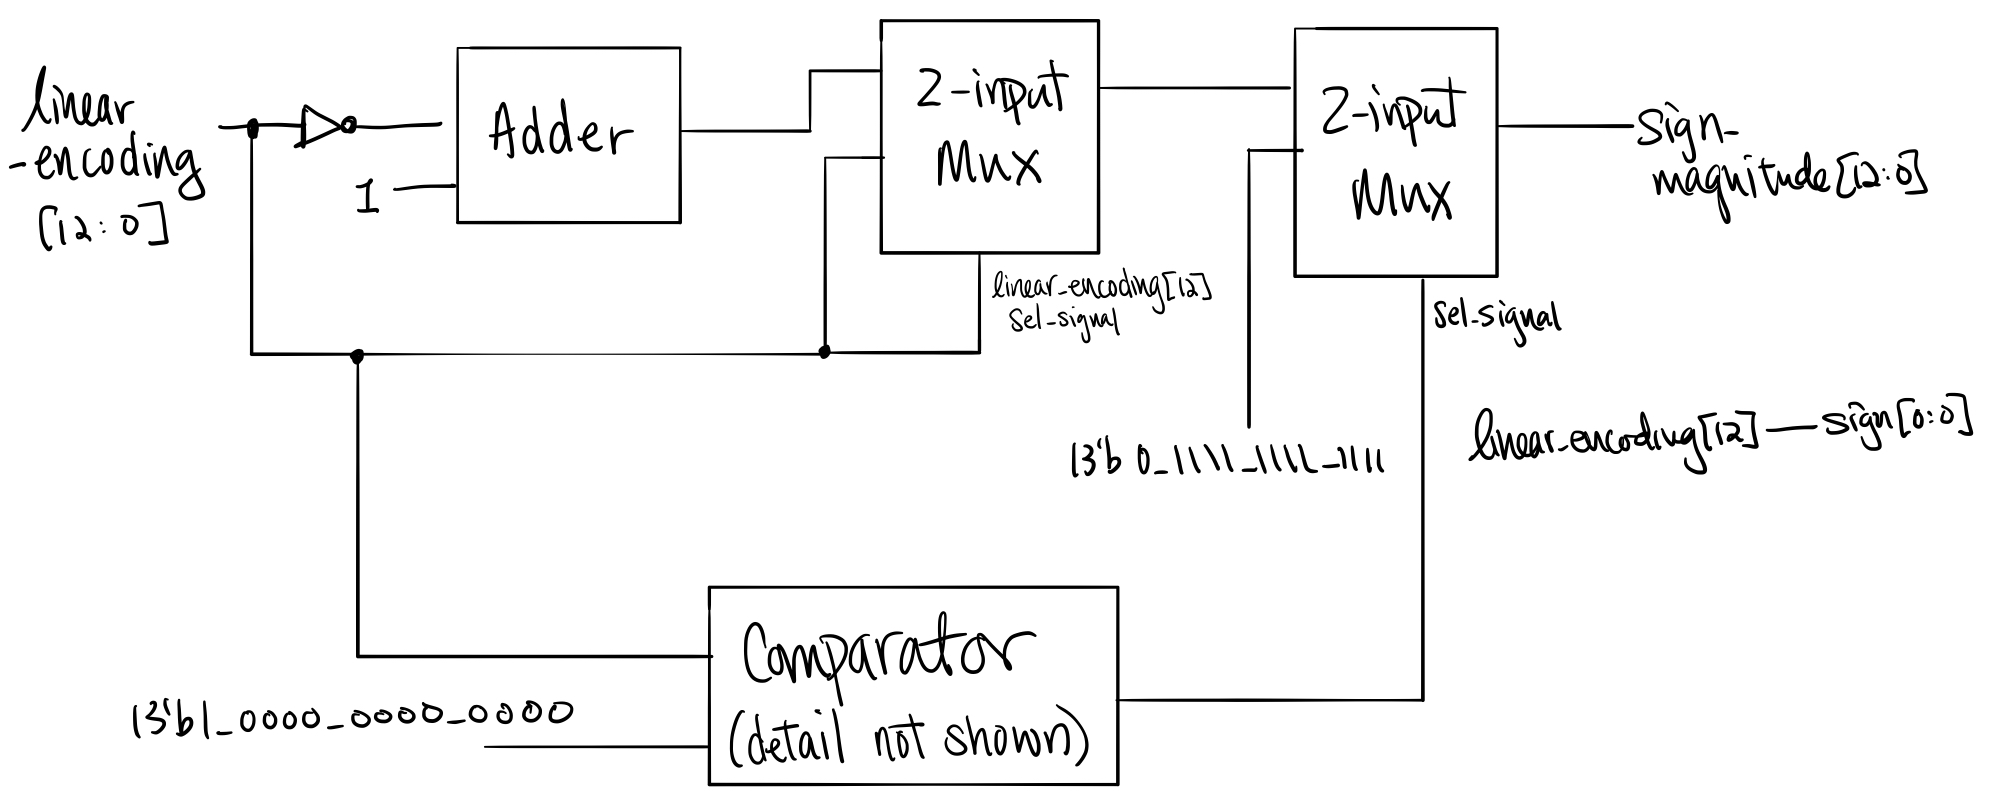
\includegraphics[scale=0.18]{module_1_schematic.jpeg} \\
    \caption{Schematic of \texttt{convertToSignMagnitude} Module}
    \end{center}
    This module will output final output \texttt{S} in our compounded 9-bit FP representation, and provide input necessary for our next module \texttt{countLeadingZeroExtractBits}.
    
    \item \textbf{Sub-Module #2: } \texttt{countLeadingZeroExtractBits} \\
    The purpose of this module is to perform the basic linear FP conversion. The exponent is computed based on counting the number of leading zeroes. The significand is the 5 bits after the leading zeroes and sixth bit is the bit after the significand. \par
    To implement this in Verilog, I designed my module to take in \texttt{[12:0] signMagnitude} computed from \texttt{convertToSignMagnitude} and my module outputs \texttt{[2:0] exponent}, \texttt{[4:0] significand}, and \texttt{sixth\_bit}. To extract the exponent, I used the idea of a priority encoder. To implement the priority encoder in Verilog, I used an \texttt{always} block with if statements testing in which bit the first 1 appears. Depending on where the leading zeroes end, I extract the \texttt{significand} and the \texttt{sixth\_bit}. \par
    A hand drawn schematic of \texttt{countLeadingZeroExtractBits} with different components, such as Priority Encoder, Shift Right, and subtractor, is shown below. The Shift Right operator is used in the diagram below to extract the outputs, but it is not actually used in the Verilog code as \texttt{significand} can be directly extracted with the corresponding index from \texttt{signMagnitude} in each if statement in the \texttt{always} block.
    \begin{center}
    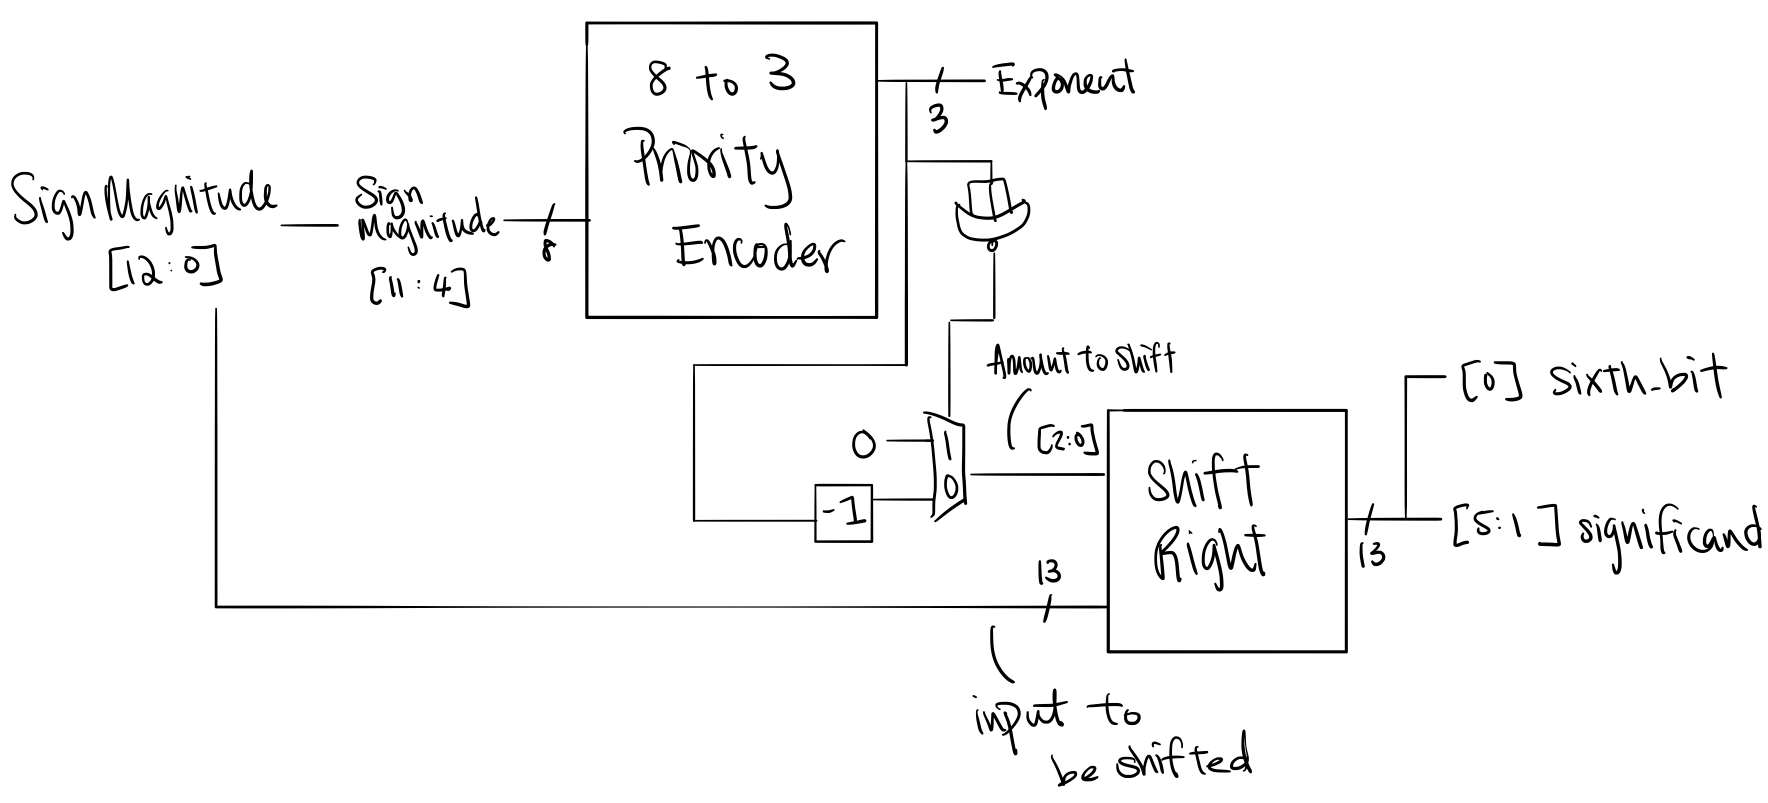
\includegraphics[scale=0.18]{module_2_schematic.jpeg} \\
    \caption{Schematic of \texttt{countLeadingZeroExtractBits} Module}
    \end{center}
    This module will output 3 outputs \texttt{exponent}, \texttt{significand}, and \texttt{sixth\_bit} used as inputs to the third sub-module \texttt{round}.
    
    \item \textbf{Sub-Module #3: } \texttt{round} \\
    The third sub-module performs rounding of the Floating Point Representation. The rounding depends on the \texttt{sixth\_bit} outputted by \texttt{countLeadingZeroExtractBits} sub-module. If \texttt{sixth\_bit  = 1}, we increment \texttt{significand} by 1. If \texttt{significand} overflows with this addition, we increase \texttt{exponent} by 1 and shift \texttt{significand} to the right by 1. \par
    To implement this sub-module in Verilog, I designed my module to take in 3 inputs \texttt{[2:0] exponent}, \texttt{[4:0] significand}, and \texttt{sixth\_bit}, and outputs \texttt{[2:0] E} and \texttt{[4:0] F}. I used an \texttt{always} block sensitive to all change, and used if statements within \texttt{always} block to check for how to proceed with calculating \texttt{E} and \texttt{F} depending on values of the three inputs. The if statements allow me to detect and take care of edge cases where either the \texttt{exponent} or \texttt{significand} will overflow if 1 is added. \par
    A hand drawn schematic of \texttt{round} is shown below, which uses components such as comparators, shift right, adders, and mux. Mux is used to represent the if statements in our Verilog code. 
    \begin{center}
    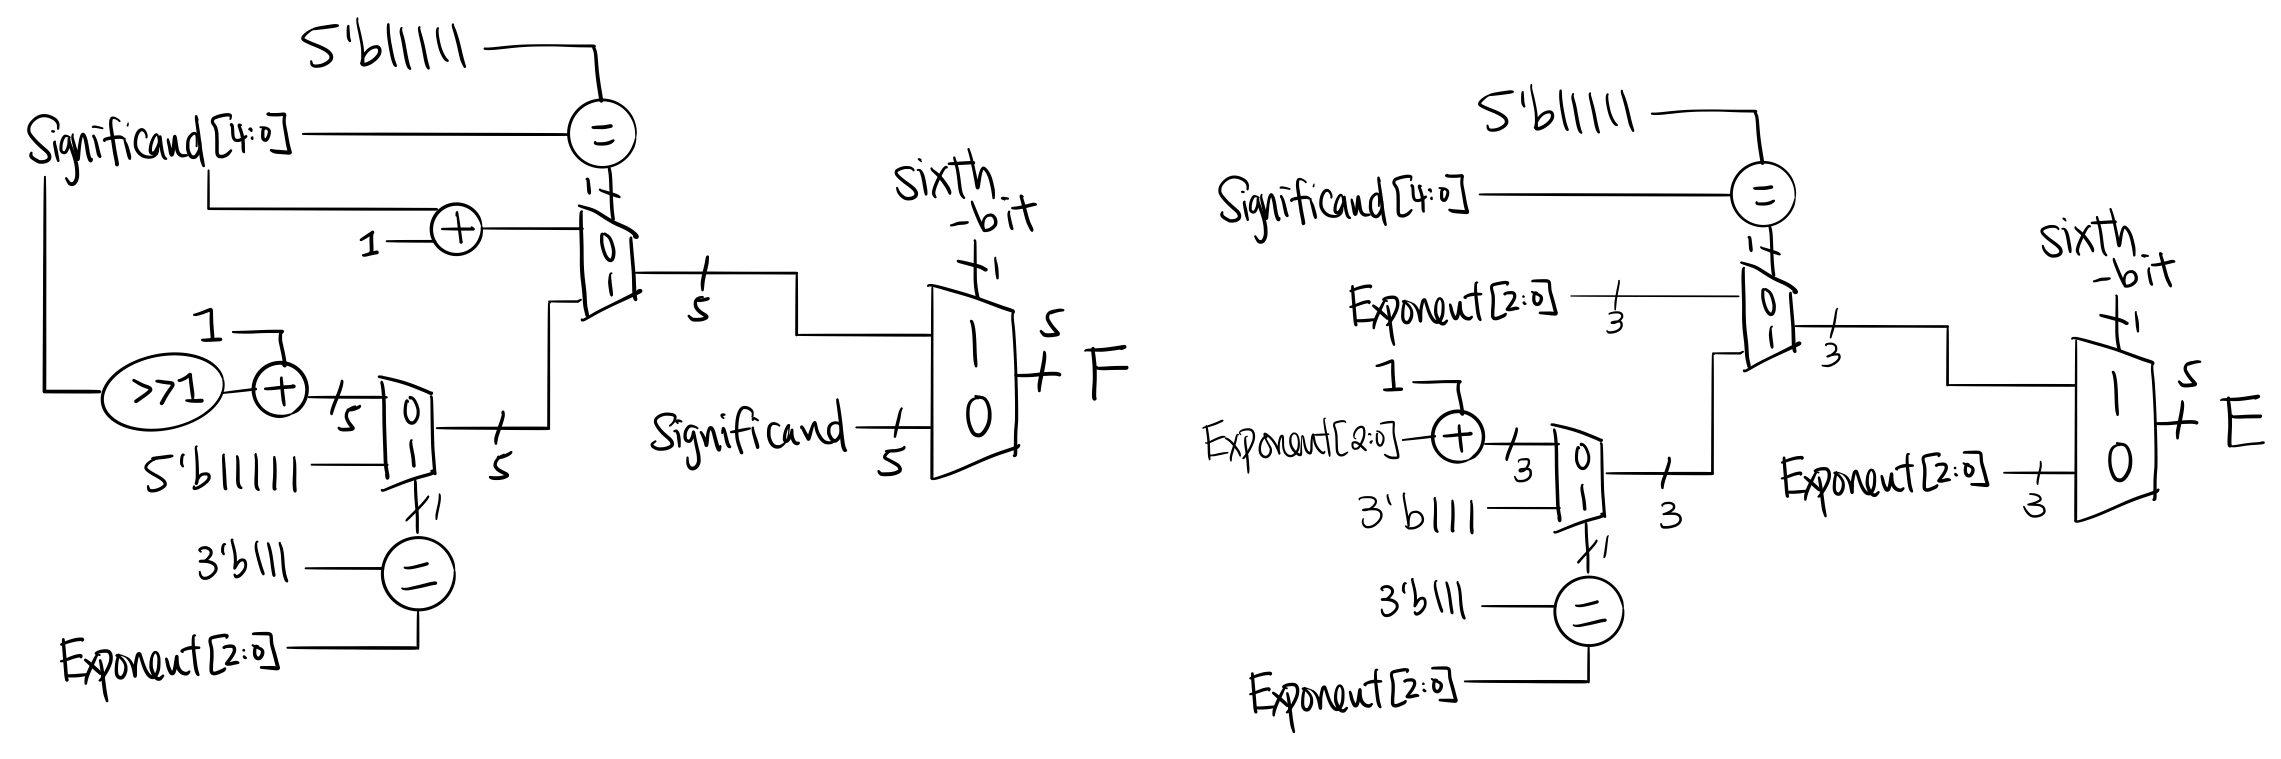
\includegraphics[scale=0.18]{module_3_schematic.jpg} \\
    \caption{Schematic of \texttt{round} Module}
    \end{center}
    The two outputs of this sub-module \texttt{E} and \texttt{F} corresponds to final outputs of our floating point conversion circuits. \texttt{E} represents the exponent while \texttt{F} represents the significand.
\end{enumerate}

\section{Simulation Documentation}
To test whether the floating point converter we implemented outputs the correct conversion, I first simulated the behavior of each sub-module and then finally simulated behavior of our combined top module.
\begin{enumerate}
    \item \textbf{Sub-Module #1: } \texttt{convertToSignMagnitude} \\
    For the \texttt{convertToSignMagnitude} module, in my test bench I tested different values of \texttt{linear\_encoding [12:0]} and observed how they change the value of output \texttt{sign} and \texttts{sign\_magnitude}. For example, when \texttt{linear\_encoding [12:0] = 0}, according to our implementation, the output \textttt{sign} should be 0 and the output \texttts{sign\_magnitude} should remain unchanged as 0 is a positive number. As shown in the first 100ns of the simulation waveform, when \texttt{linear\_encoding [12:0] = 0}, \textttt{sign = 0} and \texttts{sign\_magnitude = 0}. At 200ns, I tested the edge case where \texttt{linear\_encoding [12:0] = 1\_0000\_0000\_000}, the most negative number we can represent in 13 bits. The output we're looking for is the most positive number we can represent \texttt{13'b 0\_1111\_1111\_1111}. As shown in the simulation diagram below, indeed \textttt{sign = 1} and \texttt{sign\_magnitude = 13'b0\_1111\_1111\_1111}. At 300ns, we test yet another large magnitude negative number, and see that the output is correctly represented by value of \textttt{sign} and \texttts{sign\_magnitude}.
    
    \begin{center}
        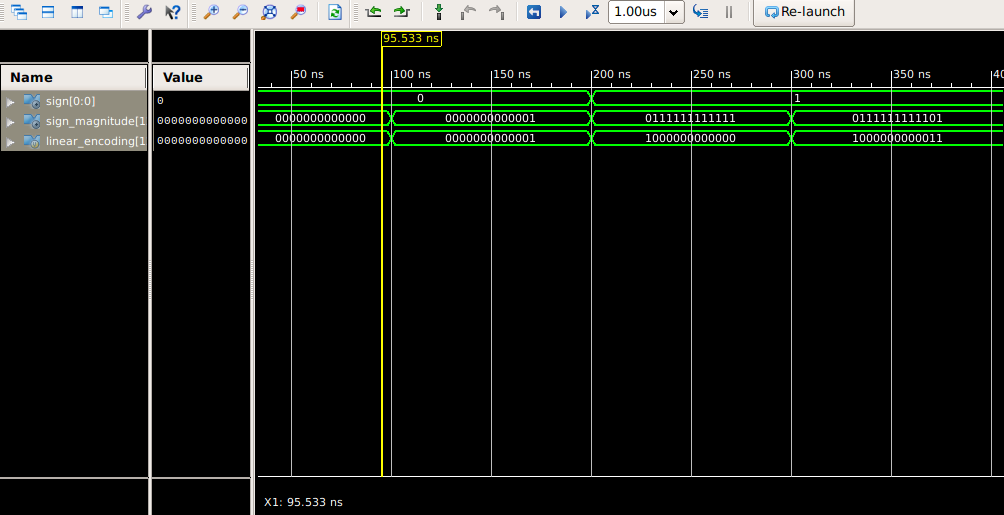
\includegraphics[scale=0.4]{sim1.png} \\
        \caption{Simulation Waveform for \texttt{convertToSignMagnitude}}
    \end{center}
    \par
    
    \item \textbf{Sub-Module #2: } \texttt{countLeadingZeroExtractBits} \\
    For this sub-module, my test bench uses different value of the \texttt{signMagnitude} input and observes how the three outputs \texttt{significand}, \texttt{sixth\_bit}, and \texttt{exponent} changes.
    \begin{center}
        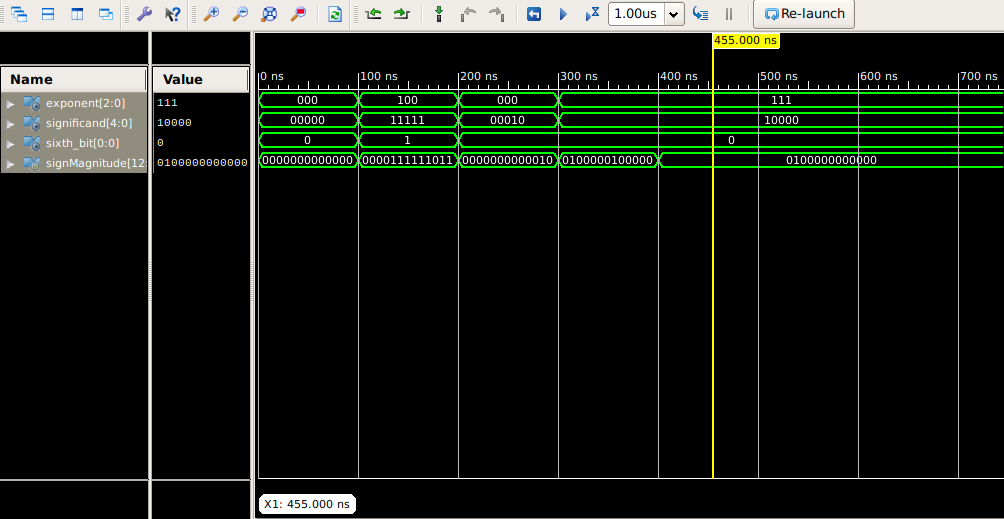
\includegraphics[scale=0.4]{sim2.png} \\
        \caption{Simulation Waveform for \texttt{countLeadingZeroExtractBits}}
    \end{center}
    From the waveform diagram above, we can see that at 0ns, \texttt{signMagnitude = 0}, so all of our outputs should be zero, which matches the output above. At 100ns, we set \texttt{signMagnitude = 13'b0\_0000\_1111\_1101}. The number of leading zeroes in this case is 5, so \texttt{exponent} should have value of 3. The 5 bits after leading zeroes are \texttt{5'b11111}. The bit after the 5 bits is \texttt{1}. This matches the output shown above. At 300ns, I tested whether our implementation can correctly extract the highest value \texttt{3'b111} when \texttt{signMagnitude = 13'b0\_1000\_0010\_0000}. At 300ns, \texttt{exponent = 111} and all the other output is correct as well, showing that our sub-module can correctly extract \texttt{significand}, \texttt{sixth\_bit}, and \texttt{exponent}.  \par

    \item \textbf{Sub-Module #3: } \texttt{round}  \\
    For this sub-module, my test bench uses different value of the 3 inputs \texttt{significand}, \texttt{sixth\_bit}, and \texttt{exponent} and observes how the two outputs \texttt{E}, and \texttt{F} changes.
    \begin{center}
        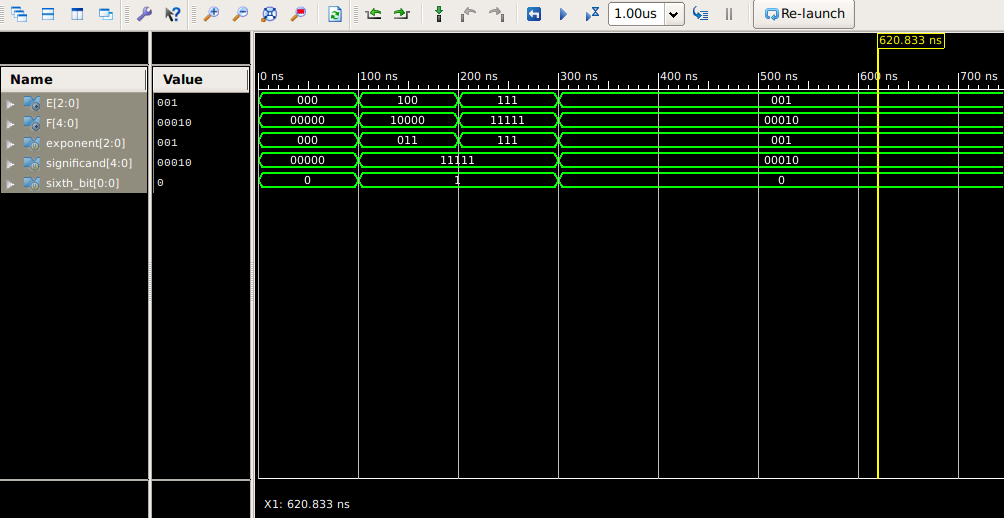
\includegraphics[scale=0.4]{sim3.png} \\
        \caption{Simulation Waveform for \texttt{round}}
    \end{center}
    From the waveform diagram above, we can see that at 0ns, all our inputs equal 0, showing that there is no need for rounding, so all of our outputs should be zero, which is true. At 100ns, we test for the edge case where we need to round up and \texttt{significand} will overflow, so \texttt{exponent} needs to be incremented. From diagram above, we clearly observe output \texttt{E} to be one higher than input \texttt{exponent} and output \texttt{F} is incremented by 1 and correctly shifted to the right by 1. At 200ns, we test for the next edge case where both \texttt{significand} and \texttt{exponent} overflows. In this case, we expect output \texttt{E} and \texttt{F} to be the largest it can be. Indeed, \texttt{E} and \texttt{F} are all 1s. At 300ns, we test the case where there is no need to round up as \texttt{sixth\_bit = 0}. \texttt{E} and \texttt{F} retains value of \texttt{significand} and \texttt{exponent} as shown in the diagram above. \par
    
    \item \textbf{Top Module: } \texttt{FPCVT}  \\
    To test to see if my top module \texttt{FPCVT} which connects the above 3 sub-modules correctly converts a linear encoding into our 9-bit compound FP representation, I used different values for input \texttt{D} and observes the change in output \texttt{S, E, D}.\par
    The wave form from my test bench is shown below:
    \begin{center}
        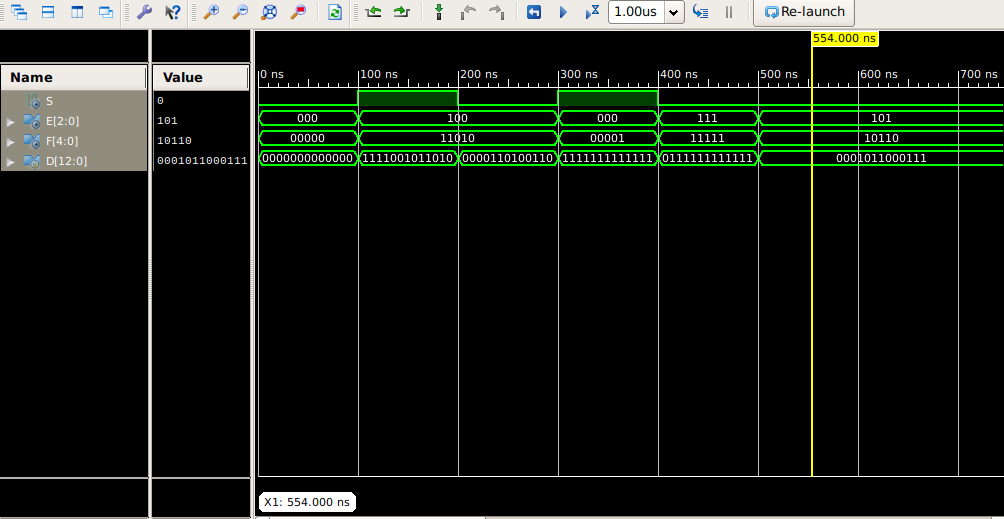
\includegraphics[scale=0.4]{sim4.png} \\
        \caption{Simulation Waveform for \texttt{FPCVT}}
    \end{center}
    At 100ns, the input \texttt{D = 13'b1\_1110\_0101\_1010} Since it is negative number, we see that \texttt{S = 1}. Once converted to 2's complement \texttt{13'b0\_0001\_1010\_0110}, we find that it has 4 leading zeroes and there is no need to round. The value of \texttt{E} should then be \texttt{3'b100}, which matches what is shown in the diagram. Since there is no need to round \texttt{F} should be \texttt{11010}, which correctly matches output in diagram. At 300ns, we test the edge case where \texttt{D} is all 1s. We correctly observe \texttt{S = 1} and \texttt{E = 0}, and \texttt{F = 1}. At 400ns, we test the edge case where \texttt{D} is the most positive number. We then correctly observe \texttt{S = 0}, and both \texttt{E} and \texttt{D} are all 1s. \par
    Some bugs I found during simulation include forgetting to increment 1 for certain roundings. I was able to fix that by trying to come up with the correct output without help of the module but with my own logic, and found the bug. \par
    \textbf{Synthesis and Implementation Report} included at end of document.
\end{enumerate}

\section{ISE Design Overview Summary Report}
\begin{center}
    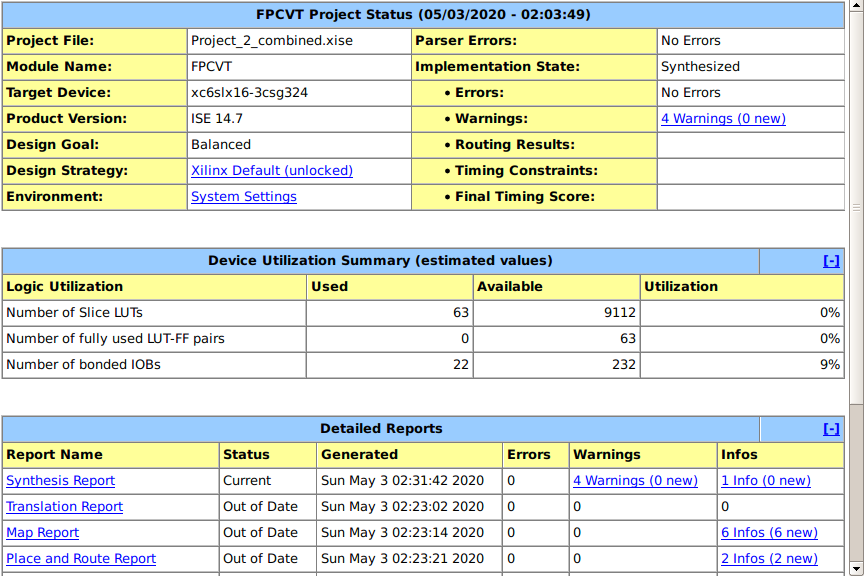
\includegraphics[scale=0.35]{design_summary.png} \\
    \caption{Design Summary}
\end{center}
My ISE Design Overview Summary Report is shown above. As you can see my implementation has no errors. There are a few warnings, but they are taken care of by my condition checking, so those cases of overflow will never occur. The resources I used can also be observed from the summary report above. 

\section{Conclusion} 
In this project, I designed and implemented the floating point converter that converts a \texttt{13'b} linear encoding of an analog signal into a compounded 9-but FP Representation. I used a lot of the knowledge learned during lecture in previous weeks to formulate my design and implement the code in Verilog. I split the task into 3 sub-modules and combined them together. Each sub-module has a smaller task so it is easier for me to design smaller individual task and then combine them together. \par
Some difficulties I encounter include deciding between when to use \texttt{wire} and \texttt{register} which often gave me bugs when I tried to synthesized. I was able to deal with this problem by looking at slides provided by TA previously about coding combinational circuits in Verilog. I also had difficulty understanding the project description but with the help and explanation of the TA, I was able to grasp full understanding. 


\newpage
\small
\section{Reports}
\subsection{Synthesis Report}
\verbatiminput{syn-report.txt}
\newpage
\subsection{Implementation Report}
\verbatiminput{imp-report.txt}

\end{document}